% Created 2021-02-07 日 10:59
% Intended LaTeX compiler: xelatex
\documentclass[11pt]{report}
\usepackage{graphicx}
\usepackage{grffile}
\usepackage{longtable}
\usepackage{wrapfig}
\usepackage{rotating}
\usepackage[normalem]{ulem}
\usepackage{amsmath}
\usepackage{textcomp}
\usepackage{amssymb}
\usepackage{capt-of}
\usepackage{hyperref}
\author{曹嘉祺 PB18030874 化学与材料科学学院 有机化学系 \thanks{中国 安徽合肥 中国科学技术大学 Email: \href{mailto:mkq@mail.ustc.edu.cn}{mkq@mail.ustc.edu.cn}}}
\usepackage[scheme=plain]{ctex}
\usepackage{fontspec}
\usepackage[section]{placeins}
\setmainfont{更纱黑体 UI SC}
\hypersetup{colorlinks=true,linkcolor=blue}
\usepackage{longtable}
\usepackage{amsmath,amsthm,amsfonts,amssymb,bm}
\usepackage{newtxtext,newtxmath}
\date{\today}
\title{电池电动势的测定及其应用}
\hypersetup{
 pdfauthor={曹嘉祺 PB18030874 化学与材料科学学院 有机化学系},
 pdftitle={电池电动势的测定及其应用},
 pdfkeywords={},
 pdfsubject={},
 pdfcreator={Emacs 27.1 (Org mode 9.3.6)}, 
 pdflang={English}}
\begin{document}

\maketitle
\tableofcontents

\begin{abstract}
本实验以银-氯化银电极为参比电极,自制铜电极、银电极和盐桥,运用对消法测量了铜-硫酸铜电极的标准电极电势,以及银-硝酸银电极的标准电极电势。根据第二个电池反应计算得到了氯化银的溶度积 K\textsubscript{sp},由其电池的电动势随温度变化曲线,根据 Nernst 方程和 Gibbs-Helmholtz 方程计算得到该反应的标准摩尔反应焓变、熵变和吉布斯自由能变化。


\noindent\rule{\textwidth}{0.5pt}
\begin{itemize}
\item 关键词:可逆电池\quad  电动势\quad  电极电势\quad  热力学函数\quad   溶度积
\end{itemize}
\end{abstract}
\begin{abstract}
In  this  experiment,  we  use  silver-silver  chloride  electrode  as  reference electrode, and  we  made  copper  electrode,  the  silver  electrode  and  the  salt  bridge  by ourselves,  with  cancellation  method  we  measured  the  standard  electrode  potential  of both the electrode of Cu-copper sulfate and the electrode of the silver-silver nitrate. According  to  the  second  battery  we  got  solubility  product  K\textsubscript{sp}  of  silver  chloride. Besides  the  curve  of  its  electromotive  force  of  the  battery  with  the  temperature, according  to  the  Nernst  equation  and  Gibbs-Helmholtz  equation  we  could  get  the standard  molar  reaction  enthalpy  change,  entropy  change  and  Gibbs  free  energy change.

\noindent\rule{\textwidth}{0.5pt}

\begin{itemize}
\item key words: Reversible Battery, EMF, Electrode, Potential, Thermodynamic Functions, the Solubility Product
\end{itemize}
\end{abstract}
\part{前言}
\label{sec:orgeea544c}

将化学反应设计成可逆电池,
通过对电池电动势的测量可以求算该反应的\(\Delta\) H,\(\Delta\) S,\(\Delta\) G 等热力学函数、
电解质的平均活度系数、难溶盐的溶度积和溶液的 pH 值等物理化学参数。
本实验就是采用对消法测电池的电动势,
从而求得AgCl 的溶度积以及该反应的标准摩尔反应焓变、熵变和吉布斯自由能变化。
\chapter{实验目的与要求}
\label{sec:org9387770}
\begin{enumerate}
\item 通过实验加深对可逆电池、可逆电极概念的理解。
\item 掌握对消法测定电池电动势的原理及电位差计的使用方法。
\item 学会一些电极和盐桥的制备。
\item 通过测量电池Ag-AgCl|KCl(m\textsubscript{1})||AgNO3(m\textsubscript{2})|Ag的电动势求AgCl的溶度积K\textsubscript{sp}。
\item 测量电池Cu|CuCl\textsubscript{2}(m\textsubscript{1})||KCl(m\textsubscript{2})|AgCl-Ag的电动势随温度的变化,并计算有关的热力学函数。
\end{enumerate}
\chapter{实验原理}
\label{sec:org490d568}
化学电池是由两个“半电池”即正负电极放在相应的电解质溶液中组成的。
由不同的这样的电极可以组成若干个原电池。
在电池反应过程中正极上起还原反应,负极上起氧化反应,
而电池反应是这两个电极反应的总和。其电动势为组成该电池的两个半电池的电极电位的代数和。
若知道了一个半电池的电极电位,通过测量这个电池电动势就可算出另外一个半电池的电极电位。
所谓电极电位,它的真实含义是金属电极与接触溶液之间的电位差。
它的绝对值至今也无法从实验上进行测定。
在电化学中,电极电位是以一电极为标准而求出其他电极的相对值。
现在国际上采用的标准电极是标准氢电极,
即在a\textsubscript{H\textsuperscript{+}}=1时,P\textsubscript{H\textsubscript{2}}=1 atm时被氢气所饱和的铂电极,
它的电极电位规定为0,然后将其他待测的电极与其组成电池,
这样测得电池的电动势即为被测电极的电极电位。
由于氢电极使用起来比较麻烦,人们常把具有稳定电位的电极,
如甘汞电极,银—氯化银电极作为第二级参比电极。

通过对电池电动势的测量可求算某些反应的\(\Delta\) H,\(\Delta\) S,\(\Delta\) G等热力学函数,
电解质的平均活度系数,难溶盐的活度积和溶液的pH等物理化学参数。
但用电动势的方法求如上数据时,必须是能够设计成一个可逆电池,
该电池所构成的反应应该是所求的化学反应。
例如用电动势法求AgCl的K\textsubscript{sp}需设计成如下的电池:
\[
   Ag-AgCl|KCl(m_{1})||AgNO_{3}(m_{2})|Ag
   \]
该电池的电极反应为:
\begin{itemize}
\item 负极反应:
\[
     Ag(s)+Cl^{-}(m_{1})\Longrightarrow AgCl(s)+e^{-}
     \]
\item 正极反应:
\[
     Ag^{+}(m_{2})+e^{-}\Longrightarrow Ag(s)
     \]
\item 电池总反应:
\[
     Ag^{+}(m_{2})+Cl^{-}(m_{1})\Longrightarrow AgCl(s)
     \]
\item 电池电动势:
\[
     E=\psi_{右}-\psi_{左}
     =[\psi^{\Theta}_{Ag^{+}/Ag}+\frac{RT}{F}\ln a_{Ag^{+}}]
     =[\psi^{\Theta}_{Ag/AgCl}+\frac{RT}{F}\ln a_{Cl^{-}}]
     \]
\[
     E=E^{\Theta}-\frac{RT}{F}\ln \frac{1}{a_{Ag^{+}}\cdot a_{Cl^{-}}}
     \]
又因为:
\[
     G^{\Theta}=-nFE^{\Theta}=-RT\ln\frac{1}{K_{sp}}
     \]
(该反应n=1),
\[
     E^{\Theta}=\frac{RT}{F}\ln\frac{1}{K_{sp}}
     \]
整理后得
\[
     E=
     \frac{RT}{F}\ln\frac{1}{K_{sp}}+\frac{RT}{F}\ln a_{Ag^{+}}\cdot a_{Cl^{-}}
     \]
\end{itemize}
\[
   E=\frac{RT}{F}\ln\frac{a_{Ag^{+}}\cdot a_{Cl^{-}}}{K_{sp}}
   =\frac{RT}{F}\ln\frac{\gamma_{\pm Ag^{+}}\cdot C_{Ag^{+}}\cdot\gamma_{\pm Cl^{-}}\cdot C_{Cl^{-}}}{K_{sp}} (C^{\Theta})^{-2}
   \]
所以只要测得该电池的电动势就可根据上式求得AgCl的K\textsubscript{sp}。
其中\(\gamma_{\pm Ag^{+}}\) 为AgNO\textsubscript{3}溶液的平均活度系数,
\(\gamma_{\pm Cl^{-}}\) 为KCl溶液的平均活度系数。
当C\textsubscript{AgNO\textsubscript{3}}=0.1000m时,
\(\gamma\)\textsubscript{\textpm{}}=0.734,C\textsubscript{KCl}=1.000m时,
\(\gamma\)\textsubscript{\textpm{}}=0.770。

化学反应的热效应可以用量热计直接度量,也可以用电化学方法来测量。
由于电池的电动势可以准确测量,
所得的数据常常较热化学方法所得的可靠。

在恒温恒压条件下,可逆电池所做的电功是最大非体积功W′,
而W′等于体系自由能的降低即为-\(\Delta\)\textsubscript{r}G\textsubscript{m}
,而根据热力学与电化学的关系,我们可得
\[
   \Delta_{r}G_{m} =-nFE
   \]

由此可见利用对消法测定电池的电动势即可获得相应的电池反应的自由能的改变。
式中的n是电池反应中得失电子的数目,F为法拉第常数。
根据吉布斯——亥姆霍茨公式
\[
   \Delta_{r}G_{m}=\Delta_{r}H_{m}-T\Delta_{r}S_{m}
   \]
\[
   \Delta_{r}S_{m}=-\left(\frac{\partial \Delta_{r}G_{m}}{\partial T}\right)_{p}=nF\left(\frac{\partial E}{\partial T}\right)_{p}
   \]

于是得到
\[
   \Delta_{r}H_{m}=-nFE+nFT\left(\frac{\partial E}{\partial T}\right)_{p}
   \]

由实验可测得不同温度时的E值,以E对T作图,
从曲线的斜率可求出任一温度下\(\left(\frac{\partial E}{\partial T}\right)_{p}\) 的值,
根据上式可求出该反应的势力学函数\(\Delta\)\textsubscript{r}G\textsubscript{m} 、\(\Delta\)\textsubscript{r}S\textsubscript{m}、\(\Delta\)\textsubscript{r}H\textsubscript{m}。
本实验测定下列电池的电动势,并由不同温度下电动势的测量求算该电池反应的热力学函数。
电池为:
\[
   Cu|CuCl_{2}(0.1000m)||Cl^{-}(1.000mKCl)|AgCl-Ag
   \]
该电池的正极反应为:
\[
   2AgCl(s)+2e^{-}\Longrightarrow 2Ag(s)+2Cl^{-}
   \]
负极反应为:
\[
   Cu(s)\Longrightarrow Cu^{2+}+2e^{-}
   \]
总电池反应为:
\[
   2AgCl(s)+Cu(s)\Longrightarrow 2Ag(s)+Cu^{2+}+2Cl^{-}
   \]
各电极电位为:
\[
   \psi_{右}=\psi^{\Theta}_{Ag,AgCl,Cl^{-}}+\frac{RT}{2F}\ln\frac{a_{AgCl}}{a^{2}_{Cl^{-}}}
   =\psi^{\Theta}_{Ag,AgCl,Cl^{-}}+\frac{RT}{2F}\ln\frac{1}{a^{2}_{Cl^{-}}}
   \]

\[
   \psi_{右}=\psi^{\Theta}_{Cu^{2+},Cu}+\frac{RT}{2F}\ln\frac{a_{Cu^{2+}}}{a_{Cu}}=
   \psi^{\Theta}_{Cu^{2+},Cu}+\frac{RT}{2F}\ln a_{Cu^{2+}}
   \]

实验中可以准确测量不同温度的E值,便可计算不同温度下该电池反应的\(\Delta\)\textsubscript{r}G\textsubscript{m}。
以E对T作图求出某任一温度的\(\left(\frac{\partial E}{\partial T}\right)_{p}\) 便可计算该温度下的\(\Delta\)\textsubscript{r}S\textsubscript{m},由\(\Delta\)\textsubscript{r}G\textsubscript{m}和\(\Delta\)\textsubscript{r}S\textsubscript{m}可求出该反应的\(\Delta\)\textsubscript{r}H\textsubscript{m}。

\part{实验部分}
\label{sec:org34a3efc}
\chapter{实验仪器与试剂}
\label{sec:orgf6c3b39}
\section{仪器}
\label{sec:org1a1468d}
\begin{center}
\begin{tabular}{lll}
仪器 & 数目 & 厂家\\
\hline
HK-2A超级恒温水浴 & 1 & 南京南大万和科技有限公司\\
EM-3D型电位差计 & 1台 & 南京南大万和科技有限公司\\
铂电极 & 2支 & \\
恒温槽 & 1套 & \\
半电池管 & 2支 & \\
U型管 & 2支 & \\
检流计 & 1只 & \\
导线若干 &  & \\
银氯化银参比电极 & 1支 & \\
铜电极 & 2支 & \\
标准电池 & 1只 & \\
毫安表、电阻箱 & 各1只 & \\
直流稳压电源 & 1台 & \\
琼脂、KCl、KNO3(分析纯) &  & \\
0.1mol\(\cdot\) dm\textsuperscript{-3} AgNO\textsubscript{3}溶液 &  & \\
0.1mol\(\cdot\) dm\textsuperscript{-3} CuCl\textsubscript{2}溶液 &  & \\
滤纸若干 &  & \\
\end{tabular}
\end{center}





\chapter{实验步骤}
\label{sec:org66b012e}
\section{制备Cu Ag电极}
\label{sec:orgd4c8186}
\begin{enumerate}
\item 银电极
\label{sec:org9f43278}
\begin{enumerate}
\item 将银电极放在浓HNO\textsubscript{3}中稍微浸泡1-2 min(可以略去),用细晶相砂纸打磨光亮,再用蒸馏水冲洗干净插入盛0.1000 M AgNO3溶液的小烧杯中,按图6-2接好线路,调节可变电阻,使电流在3 mA、直流稳压源电压控制在9 V镀20 min。
\item 取出后用蒸馏水冲洗,用滤纸吸干(冲洗以及吸干操作要以不破坏电极表面镀层为准),并迅速放入盛有0.1000 M AgNO\textsubscript{3}溶液的半电池管中
\end{enumerate}

\item 铜电极
\label{sec:org3f7e3dd}
\begin{enumerate}
\item 将铜电极放入稀硝酸中浸泡10 min,用水冲洗干净并擦干,再将待镀阴极铜棒用细晶相砂纸打磨光亮,阳极铜棒用粗砂纸稍稍打磨除去铜绿即可,用蒸馏水冲洗干净后用滤纸擦干,插入盛有铜电镀液的试剂瓶中,按步骤1中的方式,控制电流在3 mA、电压在12 V镀20 min。
\item 取出被镀电极后用蒸馏水冲洗,用滤纸吸干表面水后,放入0.1000 M的CuCl\textsubscript{2}溶液的半电池管中。
\end{enumerate}
\end{enumerate}

\section{制备盐桥}
\label{sec:org5f5a91c}
\begin{enumerate}
\item 3.0 g琼脂粉 + 120 mL饱和硝酸钾溶液(加少量KNO3晶体)到三角锥型瓶,水浴加热(防糊),搅拌使琼脂粉溶解
\item U型玻璃管预热(防止热琼脂-KNO3饱和溶液冷凝造成气泡断路)
\item 用滴管吸取热琼脂-KNO3饱和溶液缓慢加入到热U型玻璃管中直至完全充满,不能有气泡,放置自然冷却
\item 冷却后,再滴上一滴热溶液,使管口呈凸面,防止盐桥使用时在管口产生气泡
\end{enumerate}
\section{电池电动势的测量}
\label{sec:org09429c3}
\begin{enumerate}
\item 组装电池:将半电池管用蒸馏水洗净并用半电池液润洗3次,置于恒温槽中水浴,将上述制备的银电极与铜电极以及Ag/AgCl参比电极分别放入对应的半电池液中。将自制的KNO3盐桥插在待测定的两半电池管的小口上。
\item 校准电位差计:用EM-3D型电位差计测量电池的电动势,该仪器最大测量范围为1.91110 V。
\begin{enumerate}
\item 自身零点校正:模式拨至“外标”挡,调零电压,表笔短接,调零电流,
\item 标准电池校正:红黑表笔分别与标准电池的正负极相接,调节电压旋钮与给出的标准电池的电动势值相同,调零电流
\item 测量:模式拨至“测量”挡,调节电压旋钮,使检流计指示为0,此时的读数就是所测电池的电动势。
\end{enumerate}
\item 测量待测电池电动势:将上述制备的银电极与制备好的铜电极组成电池,其置于恒温槽中,将KNO\textsubscript{3}盐桥横插在两半电池管的小口上,将恒温槽置于30\textsuperscript{o}C,恒温10-15min后测量电池的电动势。
\item 测量待测E-T关系:将上述制备的银电极与实验室提供的参比电极Ag-AgCl组成电池,将自制的KNO\textsubscript{3}盐桥横插在两半电池管的小口上,分别在30\textsuperscript{o}C、35\textsuperscript{o}C、40\textsuperscript{o}C、45\textsuperscript{o}C稳定温度(恒温5min)下测量该电池的电动势。
\end{enumerate}
\chapter{实验数据及数据处理(见附件)}
\label{sec:org7141ad8}
\chapter{结果分析与讨论}
\label{sec:org35e01c1}
\section{实验结果}
\label{sec:org996af14}
\begin{enumerate}
\item 铜银电极的电极电势
\label{sec:org11e651c}
实验测得的电动势为0.4425V, 根据计算得到的标准值为0.4443V,相对误差为
\[
     \eta \%= \frac{0.4443-0.4425}{0.4443}\times 100 \%= 0.4\%
     \]
\item 氯化银电池的热力学函数计算
\label{sec:org58c4e7a}
根据测量得到的电动势对温度作图如下
\begin{center}
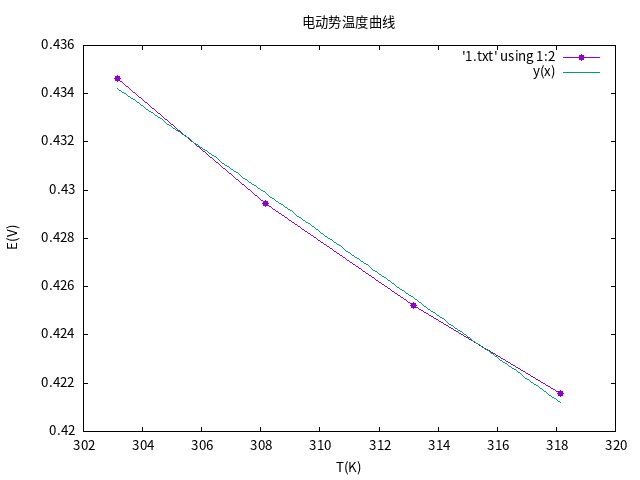
\includegraphics[width=.9\linewidth]{../data/E-T.png}
\end{center}
拟合结果为:
\[
     E=-0.0008690\times T+0.6977
     \]
根据斜率得
\[
     \left(\frac{\partial E}{\partial T}\right)_{p}=-0.0008690
     \]
由此计算出本反应的热力学函数
\[
     \Delta_{r}S_{m}=nF\left(\frac{\partial E}{\partial T}\right)_{p}=96485\times (-0.0008690)= -83.85J\cdot K^{-1}\cdot mol^{-1}
     \]
\[
     \Delta_{r}G_{m}=-nFE=-96485\times 0.43426 =-41.90kJ\cdot mol^{-1}
     \]
\[
     \Delta_{r}H_{m}=-nFE+nFT\left(\frac{\partial E}{\partial T}\right)_{p}=-67.32kJ\cdot mol^{-1}
     \]
根据文献中查到的303.15K下的标准Ksp计算出以上函数的标准值
查文献得303.15K下有:
\[
     K_{sp}=3.89\times 10^{-10}
     \]
所以:
\[
     \Delta_{r}G_{m}(303.15K)=-RT\ln (K_{sp})^{-1}=-54.61kJ\cdot mol^{-1}
     \]
考虑到熵变随温度的变化在5\textsuperscript{o}C的范围内很小可以忽略,查文献得
\[
     \Delta_{r}S_{m}(298.15K)=-32.98J\cdot K^{-1} \cdot mol^{-1}
     \]
所以可以近似地套用
\[
     \Delta_{r}S_{m}(303.15K)=-32.98J\cdot K^{-1} \cdot mol^{-1}
     \]
所以
\[
     \Delta_{r}H_{m}(303.15K)=\Delta_{r}G_{m}+T\Delta_{r}S_{m}=-64.61kJ\cdot mol^{-1}
     \]
误差如下:
\begin{center}
\begin{tabular}{lrrr}
热力学数据 & 测量值 & 理论值 & 误差(\%)\\
\hline
\(\Delta\)\textsubscript{r}G\textsubscript{m} & -41.90 & -54.61 & 23.274126\\
\(\Delta\)\textsubscript{r}H\textsubscript{m} & -67.32 & -64.61 & -4.1943972\\
\(\Delta\)\textsubscript{r}S\textsubscript{m} & -83.85 & -32.98 & -154.24500\\
\end{tabular}
\end{center}
\item 计算氯化银303.15K下的K\textsubscript{sp}
\label{sec:orgc68f1ca}
\[
     K_{sp}=3.36\times 10^{-10}
     \]
查阅文献得303.15K下理论值为
\[
     K_{sp}=3.89\times 10^{-10}
     \]
误差为:
\[
     \eta\% = \frac{3.89\times 10^{-10}-3.36\times 10^{-10}}{3.89\times 10^{-10}}\times 100\%= 15.8\%
     \]
\end{enumerate}

\section{实验讨论}
\label{sec:orgd73435c}
\begin{enumerate}
\item 本实验通过设计电池,可以通过测量的较容易得到的电池电动势来计算较难求得的热力学参数,这个转化大大简化了实验,也提高了准确度,是一种较好的物理化学实验方法。
\item 通过描绘电动势与温度的关系图,我们可以求出曲线的斜率;知道曲线斜率后,我们就可以根据计算公式得到几种热力学函数的值。这为计算反应的热力学函数提供了一种方法。
\item 我们发现随着温度的升高,溶度积常数也不断增大。这是由于对于大多数物质,随着温度升高,溶解度也增大。对于难溶物质而言,这种影响有时非常明显,甚至会是溶度积常数改变几个数量级。
\item 本实验中制作盐桥非常麻烦,非常好地锻炼了我们的实验技能
\item 误差分析:
\begin{enumerate}
\item 电位差计的读数不稳定。操作时间应尽可能的快,而且应该尽快读数,否则电极通电时间过长,电极会发生极化,给实验带来较大的误差。而实际上总是需要较长的时间才能调节仪器的到平衡,即使是同一个电动势值,在很短的时间内测得的数据都波动较大,所以这是实验的误差的来源之一。
\item 电极的电镀效果较重要。一般来说,电极表面的表面构造直接影响着电极电势的大小,所以,为了得到精确的电动势值,要保证电极特别干净,新镀上去的金属基本覆盖电极棒(即要电镀足够的时间)。
\item 本实验方法使所得数据不可能有很高的精确度,因为实验过程中取点太少,结果精确度明显不够。这也导致本次实验中直线的斜率误差很大, 直接影响了熵变的计算
\item 恒温槽温度不够稳定带来的电势随温度变化的误差。
\item 原数据点用直线拟合带来的误差。
\item AgCl 的 Ksp 的误差较大,是由于 Ksp 的值很小,而电池电动势 E 和 Ksp 是指数关系,E 测量结果对其影响很大。
\item 本实验的溶液都是实验前配制好的,其浓度可能在多次试验后由于各种原因而发生改变,并不是原来的浓度,而我们在计算时仍旧是按照最初配制的浓度,这必然会带来误差
\item 尽管我们采用了对消法测量电动势,但回路中仍存在微小的电流,这微小的电流也会产生的极化作用会破坏电池的可逆性,使电动势偏离可逆值
\item 相比于 \(\Delta\)\textsubscript{r}S\textsubscript{m} 、\(\Delta\)\textsubscript{r}G\textsubscript{m} , \(\Delta\)\textsubscript{r}H\textsubscript{m} 误差要小很多,这主要是由于\(\Delta\)\textsubscript{r} S\textsubscript{m} 值本身较小,加之实验中其它的影响因素较大,这最终导致其测量误差很大。
\end{enumerate}
\end{enumerate}







\part{参考文献}
\label{sec:org2b11ab2}
\begin{enumerate}
\item 崔献英,柯燕雄,单绍纯.物理化学实验[M].合肥:中国科学技术大学出版社,2000.4
\item 傅献彩,沈文霞,姚天扬.物理化学.第四版.北京:高等教育出版社,1990.10
\item Jimmy Xu.溶度积表[EB/OL].\url{https://zh.wikipedia.org/wiki/\%E6\%BA\%B6\%E5\%BA\%A6\%E7\%A7\%AF\%E8\%A1\%A8,2018-03-24}.
\end{enumerate}

\part{附录: 数据处理过程}
\label{sec:org5997ccc}
\chapter{原始数据}
\label{sec:org6198c13}
\section{Cu|CuCl\textsubscript{2}||AgNO\textsubscript{3}(0.1m)|Ag 电动势}
\label{sec:org15be027}

\begin{center}
\begin{tabular}{rr}
序号 & 电动势(mV)\\
\hline
1 & 441.194\\
2 & 442.834\\
3 & 443.461\\
\hline
average & 442.4963\\
\end{tabular}
\end{center}
\section{Ag-AgCl|KCl(1.0000mol\(\cdot\) kg\textsuperscript{-1})||AgNO\textsubscript{3}(0.1000mol\(\cdot\) kg\textsuperscript{-1})|Ag}
\label{sec:org265b881}

\begin{center}
\begin{tabular}{rrrrrr}
温度(\textsuperscript{o}C) & 温度(K) & 电动势1(mV) & 电动势2(mV) & 电动势3(mV) & 电动势平均(mV)\\
\hline
30.00 & 303.15 & 434.847 & 434.585 & 434.465 & 434.6323\\
35.00 & 308.15 & 429.467 & 429.365 & 429.533 & 429.4550\\
40.00 & 313.15 & 425.207 & 425.226 & 425.225 & 425.2193\\
45.00 & 318.15 & 421.608 & 421.559 & 421.514 & 421.5603\\
\end{tabular}
\end{center}

\chapter{数据处理}
\label{sec:org2010753}
\section{Cu|CuCl\textsubscript{2}||AgNO\textsubscript{3}(0.1m)|Ag 电动势}
\label{sec:org9f7a7e3}
因为:
\[
C_{AgNO_{3}}=0.1000mol\cdot dm^{3}时, \gamma_{Ag^{+}}=0.734
\]
\[
C_{CuCl_{2}}0.1000mol\cdot dm^{3}时, \gamma_{Cu^{2+}}=0.150
\]
可得
\[
\psi^{\Theta}_{Ag^{+}/Ag}(298.15K)-\psi^{\Theta}_{Cu^{2+}/Cu}(298.15K)=0.4577V
\]
所以
\[
E(303.15K)=E^{\Theta}-\frac{RT}{2F}\ln\frac{a_{Cu^{2+}}}{(a_{Ag^{+}})^2}=0.4443V
\]
相对误差为
\[
\eta \%= \frac{0.4443-0.4425}{0.4443}\times 100 \%= 0.4\%
\]
\section{Ag-AgCl|KCl(1.0000mol\(\cdot\) kg\textsuperscript{-1})||AgNO\textsubscript{3}(0.1000mol\(\cdot\) kg\textsuperscript{-1})|Ag热力学函数计算}
\label{sec:orge7ef241}

\begin{center}
\begin{tabular}{rr}
温度(K) & 电动势平均(mV)\\
\hline
303.15 & 434.6323\\
308.15 & 429.4550\\
313.15 & 425.2193\\
318.15 & 421.5603\\
\end{tabular}
\end{center}
对上表作图得
\begin{center}
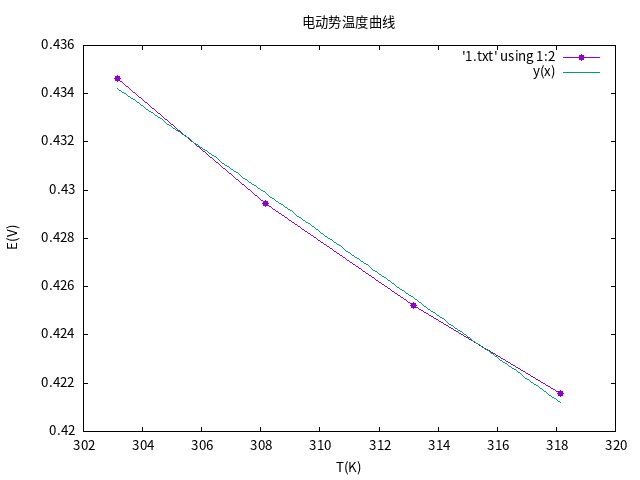
\includegraphics[width=.9\linewidth]{../data/E-T.png}
\end{center}
拟合结果如下
\begin{verbatim}
After 8 iterations the fit converged.
final sum of squares of residuals : 5.82966e-07
rel. change during last iteration : -2.04324e-13

degrees of freedom    (FIT_NDF)                        : 2
rms of residuals      (FIT_STDFIT) = sqrt(WSSR/ndf)    : 0.000539892
variance of residuals (reduced chisquare) = WSSR/ndf   : 2.91483e-07

Final set of parameters            Asymptotic Standard Error
=======================            ==========================
k               = -0.000869034     +/- 4.829e-05    (5.557%)
b               = 0.697682         +/- 0.015        (2.15%)

correlation matrix of the fit parameters:
#                k      b      
k               1.000 
b              -1.000  1.000 

\end{verbatim}
\[
E=-0.0008690\times T+0.6977
\]
\[
\left(\frac{\partial E}{\partial T}\right)_{p}=-0.0008690
\]
当T=303.15K时, E=0.43426V,
对于电池反应
\[
Ag^{+}(m_{2})+Cl^{-}(m_{1})\Longrightarrow AgCl(s)
\]
\[
\Delta_{r}S_{m}=nF\left(\frac{\partial E}{\partial T}\right)_{p}=96485\times (-0.0008690)= -83.85J\cdot K^{-1}\cdot mol^{-1}
\]
\[
\Delta_{r}G_{m}=-nFE=-96485\times 0.43426 =-41.90kJ\cdot mol^{-1}
\]
\[
\Delta_{r}H_{m}=-nFE+nFT\left(\frac{\partial E}{\partial T}\right)_{p}=-67.32kJ\cdot mol^{-1}
\]
查文献得303.15K下有:
\[
K_{sp}=3.89\times 10^{-10}
\]
所以:
\[
\Delta_{r}G_{m}(303.15K)=-RT\ln (K_{sp})^{-1}=-54.61kJ\cdot mol^{-1}
\]
考虑到熵变随温度的变化在5\textsuperscript{o}C的范围内很小可以忽略,查文献得
\[
\Delta_{r}S_{m}(298.15K)=-32.98J\cdot K^{-1} \cdot mol^{-1}
\]
所以可以近似地套用
\[
\Delta_{r}S_{m}(303.15K)=-32.98J\cdot K^{-1} \cdot mol^{-1}
\]
所以
\[
\Delta_{r}H_{m}(303.15K)=\Delta_{r}G_{m}+T\Delta_{r}S_{m}=-64.61kJ\cdot mol^{-1}
\]
\begin{center}
\begin{tabular}{lrrr}
热力学数据 & 测量值 & 理论值 & 误差(\%)\\
\hline
\(\Delta\)\textsubscript{r}G\textsubscript{m} & -41.90 & -54.61 & 23.274126\\
\(\Delta\)\textsubscript{r}S\textsubscript{m} & -83.85 & -32.98 & -154.24500\\
\(\Delta\)\textsubscript{r}H\textsubscript{m} & -67.32 & -64.61 & -4.1943972\\
\end{tabular}
\end{center}
\section{氯化银K\textsubscript{sp}计算}
\label{sec:org1f69346}
30\textsuperscript{o}C时,有
\[
    E=\frac{RT}{F}\ln\frac{a_{Ag^{+}}
    \cdot a_{Cl^{-}}}{K_{sp}}
    =\frac{RT}{F}\ln\frac{\gamma_{\pm Ag^{+}}
    \cdot
    C_{Ag^{+}}\cdot\gamma_{\pm Cl^{-}}\cdot C_{Cl^{-}}}{K_{sp}} (C^{\Theta})^{-2}
    \]
当C\textsubscript{AgNO\textsubscript{3}}=0.1000M时,
\(\gamma\)\textsubscript{\textpm{}}=0.734,
C\textsubscript{KCl}=1.000M时,
\(\gamma\)\textsubscript{\textpm{}}=0.770,

,所以有
\[
    E=\frac{RT}{F}\ln\frac{0.734
    \cdot
    0.1000
    \cdot
    0.770
    \cdot
    0.1000
    }{K_{sp}} (C^{\Theta})^{-2}=0.4346323 
    \]
则
解得
\[
    K_{sp}=3.36\times 10^{-10}
    \]
查阅文献得303.15K下理论值为
\[
    K_{sp}=3.89\times 10^{-10}
    \]
误差为:
\[
    \eta\% = \frac{3.89\times 10^{-10}-3.36\times 10^{-10}}{3.89\times 10^{-10}}\times 100\%= 15.8\%
    \]
\end{document}
